\section{Conception détaillée}

	\subsection{Diagrammes de classes}
	Les diagrammes de classes présentés dans cette partie se basent sur les diagrammes de modèle du domaine explicités précédemment.
	Ainsi les entités ont été reportées en classes, avec les fonctions qui leur sont associées.
	\begin{figure}[H]
		\centerline{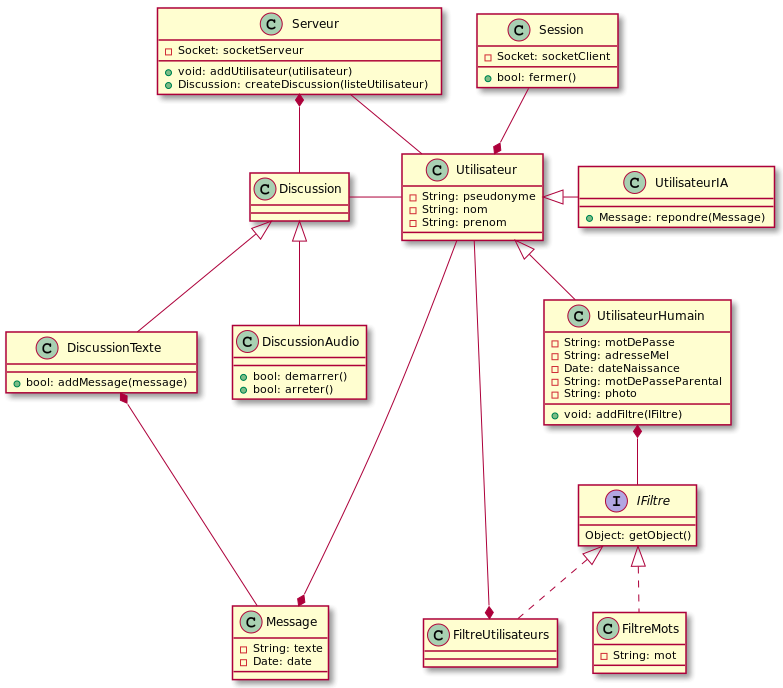
\includegraphics[width=16.5cm]{img/classesServeur.png}}
		\caption{Diagramme de classes côté serveur}
	\end{figure}

	\newpage

	Ce diagramme de classes représente la partie client de notre application, avec les attributs et méthodes des différentes classes.
	Les getter et setter ne sont pas présents sur celui-ci mais seront présents sur tout les attributs des classes Message, Discussion et Utilisateur.
	\begin{figure}[H]
		\centerline{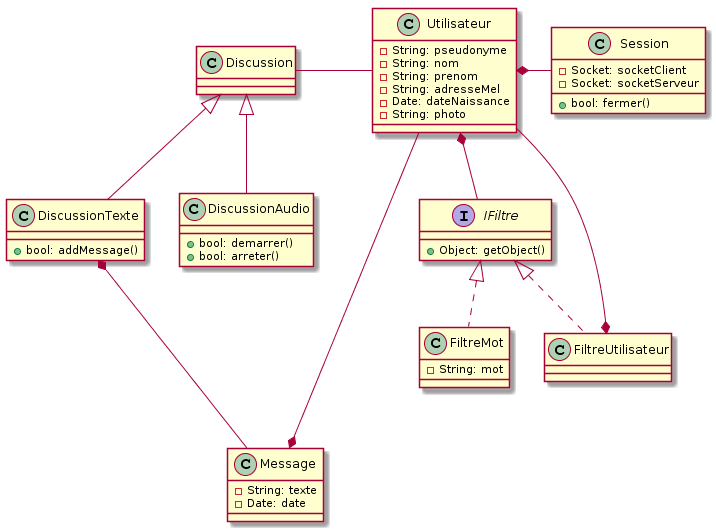
\includegraphics[width=16.5cm]{img/classesClient.png}}
		\caption{Diagramme de classes côté client}
	\end{figure}

	%% Détailler par package les élements les constituant.
	%% TODO :
	%% - Préciser les attributs et méthodes de classe de toutes les classes participantes et de les regrouper dans un diagramme de classes.

	%% Les méthodes d’un package qui seront considérée comme non triviales devront être commentées et voir leur fonctionnement détaillé par du pseudo-code.
	%
	% \begin{figure}[H]
	% 	\centerline{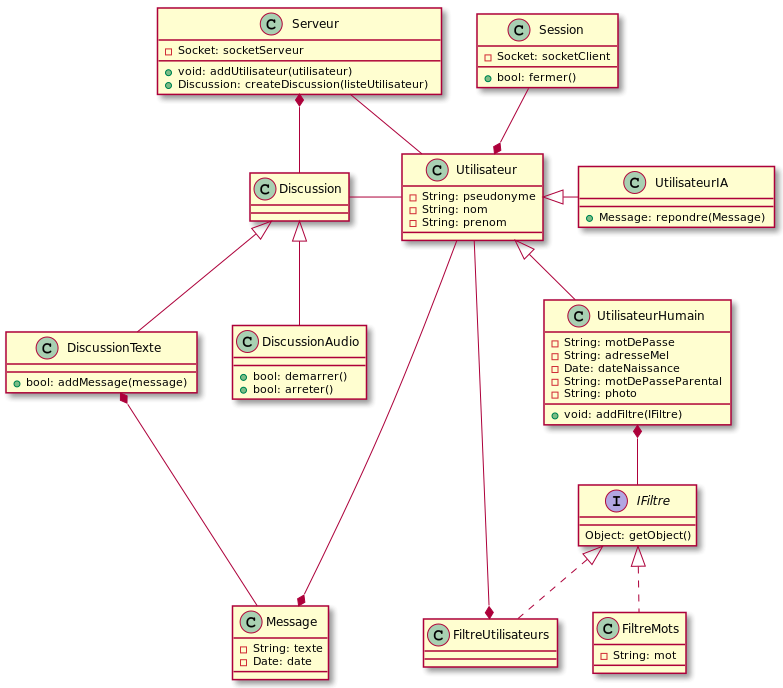
\includegraphics[width=16.5cm]{img/diagClassServeur.png}}
	% 	\caption{Diagramme de classes}
	% \end{figure}
